\renewcommand\thetable{\arabic{chapter}-\arabic{table}}
%\renewcommand\thefigure{\arabic{chapter}-\arabic{figure}}
\renewcommand{\theequation}{\arabic{chapter}-\arabic{equation}}
\chapter{資料探勘}

過往在各種不同商業、工業、學術等領域都隨著產業逐步的數位化,有各種資料庫甚至資料倉儲系統的建置與資料收集,例如零售業的交易紀錄,各種學術實驗的結果記錄等等,而隨著時間推移,這些資料庫和倉儲系統收集的資料數量都成長的非常龐大,資料間的關係和複雜度也越來越複雜,這些資料除了當初建置的目的和資料的統計分析外,研究人員還開始思考更進一步的資料應用,希望能把資料中以往隱藏不可見的知識找出來,因此資料探勘 (Data Mining) 此一研究領域就因應而生。資料探勘的方法包括統計、線上分析處理 (OLAP、on-line analytical processing)、情報檢索 (information retrieval)、機器學習 (machine learning)、模式識別 (pattern recognition) 等。

資料探勘的流程也有多種規範,其中最廣為被使用的是~CRISP-DM\cite{shearer2000crisp}(Cross Industry Standard Process for Data Mining),是由~SPSS~以及~NCR~兩大廠商在~1990年開始發展的,它的流程架構如圖~\ref{fig:CRISP-DM}~所示,將一個完整的資料探勘流程分為六個步驟,分別為:

\begin{figure}[hbtp]
  \begin{center}
    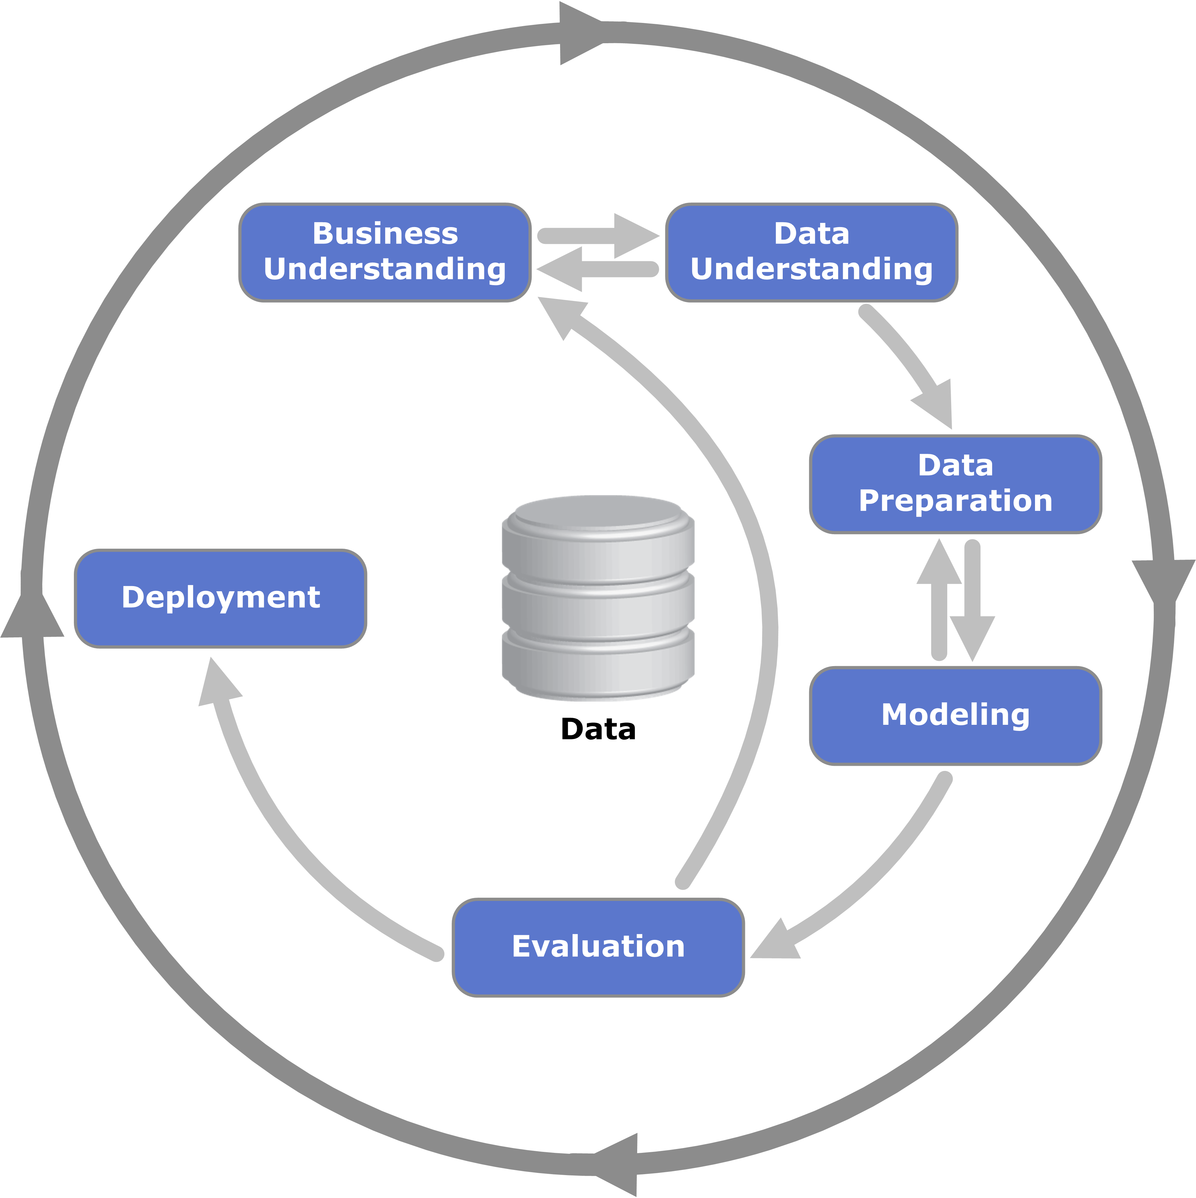
\includegraphics[width=1.0\textwidth]{figures/1196px-CRISP-DM_Process_Diagram.png}
    \caption{CRISP-DM (c)Kenneth Jensen, CC BY-SA 3.0} 
    \label{fig:CRISP-DM}
  \end{center}
\end{figure}

\begin{enumerate}
\item \textbf{定義領域問題}(Business Understanding),CRISP-DM~所定義的資料探勘最初的步驟是瞭解並定義此一資料探勘所希望解決的問題。
\item \textbf{定義分析資料}(Data Understanding),瞭解問題之後,就要定義要解答此一問題所需要的資料為何,並且著手收集。
\item \textbf{資料前處理}(Data Preparation),這個步驟包括了資料的由於現實世界的資料都會有很多雜訊在其中,因此在真正的訓練並建立模型之前,需要先把雜訊去除,包括了不合理的資料、多餘欄位,甚至是透過一些方法來凸顯資料中本來較不明顯的特定性質。
\item \textbf{建立模型}(Modeling),選擇適合該問題的資料探勘方法對前處理過的資料進行分析與模型建立。
\item \textbf{評估模型}(Evaluation),評估前一步驟中所建立的模型品質是否符合需,多是將資料分為訓練集與測試集兩組來驗證模型的可靠度。
\item \textbf{應用模型}(Deployment),將模型產出的知識實際納入應用,抑或是將探勘結果整理成完整的報告。
\end{enumerate}

本研究之流程較~CRISP-DM~之流程稍有不同,是先基於一個現有的特定領域的校舍耐震資料庫作分析,找出校舍耐震資料庫中各種潛藏知識的可能性,定義出希望能夠解決的問題,接著分析不同的問題,從校舍耐震資料庫中挑選出相關的資料屬性,然後接著進行資料前處理、建立模型、評估模型幾個步驟。

資料探勘技術方法繁多,Fayyad~\cite{fayyad1996data}根據其處理的問題形式,將資料探勘的方法分為分類、分群、迴歸尋找關聯等四種主要的問題類型,分類方法處理的問題是在用來判斷資料的類別,而且這些類別是已知的類別,例如將所有的校舍資料分類成有安全疑慮和沒有安全疑慮的就是屬於分類問題。分群問題和分類問題有點相似,一樣是將資料分成數個群組,最主要的差異是分群問題的各個群組特性一開始並不清楚,分群方法是將資料根據其屬性數值為依據,把相似的放在同一個群組,不同群組的特性是要在分出群組後進行分析才會得到。迴歸問題就是要用回歸方法來從資料的屬性中,找出特定屬性與其他屬性間的關係模型,這些屬性間的關係可能是非線性的,而且沒有解析解的關係模型,因此常見的方法是用統計回歸的方式,用現有的資料來回歸得到,又或著是用像類神經網路之類的機器學習方式,拿現有的資料下去學習已得到關係模型,以校舍耐震資料庫來說,校舍耐震能力指標的預測就是一種回歸問題,因為校舍耐震能力指標與其校舍的設計參數間的關係就是一個非線性關係,要得到兩者之間的非線性模型就需要用到回歸問題的處理方法,回歸問題也是最常見的資料探勘問題種類。最後一種是尋找屬性間的關聯,這種問題的主要目標在尋找不同筆資料屬性間所存在的關係,舉例來說,使用校舍耐震資料庫的資料來作關聯分析,可能可以去尋找像是:五層樓的校舍的校舍長度深度有什麼趨勢,或是民國八十到九十年之間的校舍的校舍走廊設計是否偏好有走廊柱等。本研究在確定主要的探勘目標後,使用的資料探勘方式為迴歸為主,分類分群為輔助。

以下分別介紹本研究所使用到的各種分析方法,除建立模型的各種訓練和演算法外,還包括資料前處理和驗證所使用的分析方法和驗證指標。


\section{資料前處理方法}

資料前處理方法常見的目的有:找出重要性較高的屬性、凸顯資料特性、剔除特異資料點等;本研究主要的資料過濾方法為資料的合理性分析,因此使用的前處理方法較少,只有主成分分析法。

\subsubsection{主成分分析}

PCA, a very common data preparation method, can identify very important attributes among various attributes. The goal is to convert the original variables through vector transition into mutually independent variables of a linear combination. The ideal situation is that principal components obtained from linear combination retain most of the information of original variables.

\section{資料探勘方法}

資料探勘的方法分為分類、分群、迴歸尋找關聯~\cite{fayyad1996data},其中迴歸是最常使用到的一種,本研究的主要目標皆可以歸納為迴歸類的問題,因此使用到的迴歸演算法最多,接著才是作為輔助用的分類和分群演算法。

\subsection{迴歸方法}

\subsubsection{Generalized Linear Model}

廣義線性模型是由Nelder and Wedderburn~\cite{citeulike:5485398}所提出,比起迴歸分析(simple regression)更為彈性,此模型是假設資料點的分佈有一分佈模式,且X與Y之間的關係是由一連結函數(Link Function)建立,如log function、power function等,其定義之XY關係模型如下:


\begin{equation} g(E(y)) = x\beta + O, y~F \label{eq:GLM}\end{equation} 

$g(.)$是為所選的鏈結函數,O是偏移(offset)變數,F則是y的分佈模型,其是用牛頓法(Newton-Raphson Method)不斷的調整$\beta$使的$x\beta + O$逼近$g(E(y))$,最後最接近的方程式即為XY兩者的關系式。比起迴歸分析,此方法還需要了解Y值分佈狀況,選擇出最適合的分佈函數,並假設XY間的鏈結函數形式,雖然越多的參數選擇代表了更多的模型不確定性,但廣義線性模型卻能夠提供比迴歸分析更廣的應用範圍,也可能得到更接近真實的關係模型。

\subsubsection{Support Vector Machine}

SVM最早是BOSER~\cite{boser1992}等人,在1992年的COLT (Computational Learning Theory)所提出,SVM是一個基於統計學習理論的分類方法,用來處理二元分割的問題,其原理是將原本無法線性分割的問題轉換到一個不同維度的空間(kernel)後,假設該空間存在一超平面(hyperplane),可以正確的將資料分開,並將尋找此一超平面的問題轉換為一最佳化問題,求解後即可得到二元分割邊界的方程式。而後Harris Drucker, et. al.,[9] 將此二元分割問題轉換為迴歸分析問題,故SVM也可以處理迴歸問題。

\subsubsection{Artificial Neural Networks}

其是希望能模擬建構出人腦內的神經網路,以處理各種複雜的問題,人類大腦是由大約千兆個神經元(Neuron)所構成,而每個神經元又會和其他約一萬個神經元連結,構成一個龐大且複雜的神經網路,這樣複雜的一個神經網路讓人類可以學習並了解各種事物與知識。McCulloch and Pitts~\cite{mcculloch1943logical}所提出的模型為後續類神經網路發展的雛形,一個標準的類神經網路可以分為輸入層(input layer)、隱藏層(hidden layer)、輸出層(output layer),輸入層(input layer)負責接受各種求解問題需要的量化數據和資料,經由隱藏層(hidden layer)的不斷自我更新學習的模型處理過後,在輸出層(output layer)就可以得到想要的解答,類神經網路可以處理的問題種類多樣,其模型的品質多數也都不錯,缺點是學習時間長,且得到的模型為一個黑盒子,難以解釋其物理或是數學模型上的意義。

\subsubsection{Genetic Programming}



\subsubsection{Weighted Genetic Programming}


\subsection{分類方法}

\subsubsection{Two-Step Classification}

Based on of the massive volume of basic data for school build- ings in the database, this study chooses two-step clustering method. The basic concept was first proposed by Zhang, Ramakrishnan and Livny~\cite{zhang1996birch} for handling large amounts of data. This method has two major steps. The first step sequences data and pre-clusters sequences into small subclusters based on the similarity of adjacent data, thereby reducing the amount of data. The second step divides several small subclusters into the desired number of clusters using a hierarchical clustering method. The hierarchical clustering method then combines close subclusters slowly until the stop condition is met. The computing speed of this method is influenced slightly by the volume of data.


\subsection{分群方法}

\subsubsection{K-means}

As proposed by MacQueen~\cite{macqueen67}, K-means is one of the most common clustering methods and has a wide application scope. Notably, it is a machine learning method; its principal steps are as follows.

\begin{enumerate}
\item A user indicates that data should be grouped into K clusters.
\item Data are divided randomly and equally into K groups and the center of each cluster are calculated.
\item Each bit of data should find the proximal center of a cluster and update its cluster label that it belongs to.
\item Recalculate the new cluster center.
\item Repeat steps 3 to 4 until the cluster centers of all data do not change.
\end{enumerate}


\section{探勘結果驗證方法與指標}



\subsection{驗證方法}

\subsubsection{10 fold cross validation}


\subsection{結果指標}

\subsubsection{決定係數 Coefficient of determination}

$R^2$

\subsubsection{平均絕對百分比誤差 MAPE}

Mean Absolute Percentage Error

\subsubsection{均方根誤差 RMSE}

均方根誤差(Root Mean Squared Error,RMSE)定義如下:

\begin{equation} RMSE = \sqrt{\dfrac{\sum{(y_i - \hat{y_i})^2}}{N}} \label{eq:RMSE}\end{equation}

其中~$N$~是資料的總數,~$y$~是透過資料所建立的關係模型所求得的輸出屬性預測值,~$\hat{y}$~則是輸出屬性的實際值,此一指標代表了模型產出結果的平均誤差,越小越好,其可接受範圍則要根據輸出屬性的數量級和問題複雜度而定。


\subsubsection{命中率 Hit Rate}





